\documentclass[1p]{elsarticle_modified}
%\bibliographystyle{elsarticle-num}

%\usepackage[colorlinks]{hyperref}
%\usepackage{abbrmath_seonhwa} %\Abb, \Ascr, \Acal ,\Abf, \Afrak
\usepackage{amsfonts}
\usepackage{amssymb}
\usepackage{amsmath}
\usepackage{amsthm}
\usepackage{scalefnt}
\usepackage{amsbsy}
\usepackage{kotex}
\usepackage{caption}
\usepackage{subfig}
\usepackage{color}
\usepackage{graphicx}
\usepackage{xcolor} %% white, black, red, green, blue, cyan, magenta, yellow
\usepackage{float}
\usepackage{setspace}
\usepackage{hyperref}

\usepackage{tikz}
\usetikzlibrary{arrows}

\usepackage{multirow}
\usepackage{array} % fixed length table
\usepackage{hhline}

%%%%%%%%%%%%%%%%%%%%%
\makeatletter
\renewcommand*\env@matrix[1][\arraystretch]{%
	\edef\arraystretch{#1}%
	\hskip -\arraycolsep
	\let\@ifnextchar\new@ifnextchar
	\array{*\c@MaxMatrixCols c}}
\makeatother %https://tex.stackexchange.com/questions/14071/how-can-i-increase-the-line-spacing-in-a-matrix
%%%%%%%%%%%%%%%

\usepackage[normalem]{ulem}

\newcommand{\msout}[1]{\ifmmode\text{\sout{\ensuremath{#1}}}\else\sout{#1}\fi}
%SOURCE: \msout is \stkout macro in https://tex.stackexchange.com/questions/20609/strikeout-in-math-mode

\newcommand{\cancel}[1]{
	\ifmmode
	{\color{red}\msout{#1}}
	\else
	{\color{red}\sout{#1}}
	\fi
}

\newcommand{\add}[1]{
	{\color{blue}\uwave{#1}}
}

\newcommand{\replace}[2]{
	\ifmmode
	{\color{red}\msout{#1}}{\color{blue}\uwave{#2}}
	\else
	{\color{red}\sout{#1}}{\color{blue}\uwave{#2}}
	\fi
}

\newcommand{\Sol}{\mathcal{S}} %segment
\newcommand{\D}{D} %diagram
\newcommand{\A}{\mathcal{A}} %arc


%%%%%%%%%%%%%%%%%%%%%%%%%%%%%5 test

\def\sl{\operatorname{\textup{SL}}(2,\Cbb)}
\def\psl{\operatorname{\textup{PSL}}(2,\Cbb)}
\def\quan{\mkern 1mu \triangleright \mkern 1mu}

\theoremstyle{definition}
\newtheorem{thm}{Theorem}[section]
\newtheorem{prop}[thm]{Proposition}
\newtheorem{lem}[thm]{Lemma}
\newtheorem{ques}[thm]{Question}
\newtheorem{cor}[thm]{Corollary}
\newtheorem{defn}[thm]{Definition}
\newtheorem{exam}[thm]{Example}
\newtheorem{rmk}[thm]{Remark}
\newtheorem{alg}[thm]{Algorithm}

\newcommand{\I}{\sqrt{-1}}
\begin{document}

%\begin{frontmatter}
%
%\title{Boundary parabolic representations of knots up to 8 crossings}
%
%%% Group authors per affiliation:
%\author{Yunhi Cho} 
%\address{Department of Mathematics, University of Seoul, Seoul, Korea}
%\ead{yhcho@uos.ac.kr}
%
%
%\author{Seonhwa Kim} %\fnref{s_kim}}
%\address{Center for Geometry and Physics, Institute for Basic Science, Pohang, 37673, Korea}
%\ead{ryeona17@ibs.re.kr}
%
%\author{Hyuk Kim}
%\address{Department of Mathematical Sciences, Seoul National University, Seoul 08826, Korea}
%\ead{hyukkim@snu.ac.kr}
%
%\author{Seokbeom Yoon}
%\address{Department of Mathematical Sciences, Seoul National University, Seoul, 08826,  Korea}
%\ead{sbyoon15@snu.ac.kr}
%
%\begin{abstract}
%We find all boundary parabolic representation of knots up to 8 crossings.
%
%\end{abstract}
%\begin{keyword}
%    \MSC[2010] 57M25 
%\end{keyword}
%
%\end{frontmatter}

%\linenumbers
%\tableofcontents
%
\newcommand\colored[1]{\textcolor{white}{\rule[-0.35ex]{0.8em}{1.4ex}}\kern-0.8em\color{red} #1}%
%\newcommand\colored[1]{\textcolor{white}{ #1}\kern-2.17ex	\textcolor{white}{ #1}\kern-1.81ex	\textcolor{white}{ #1}\kern-2.15ex\color{red}#1	}

{\Large $\underline{12n_{0746}~(K12n_{0746})}$}

\setlength{\tabcolsep}{10pt}
\renewcommand{\arraystretch}{1.6}
\vspace{1cm}\begin{tabular}{m{100pt}>{\centering\arraybackslash}m{274pt}}
\multirow{5}{120pt}{
	\centering
	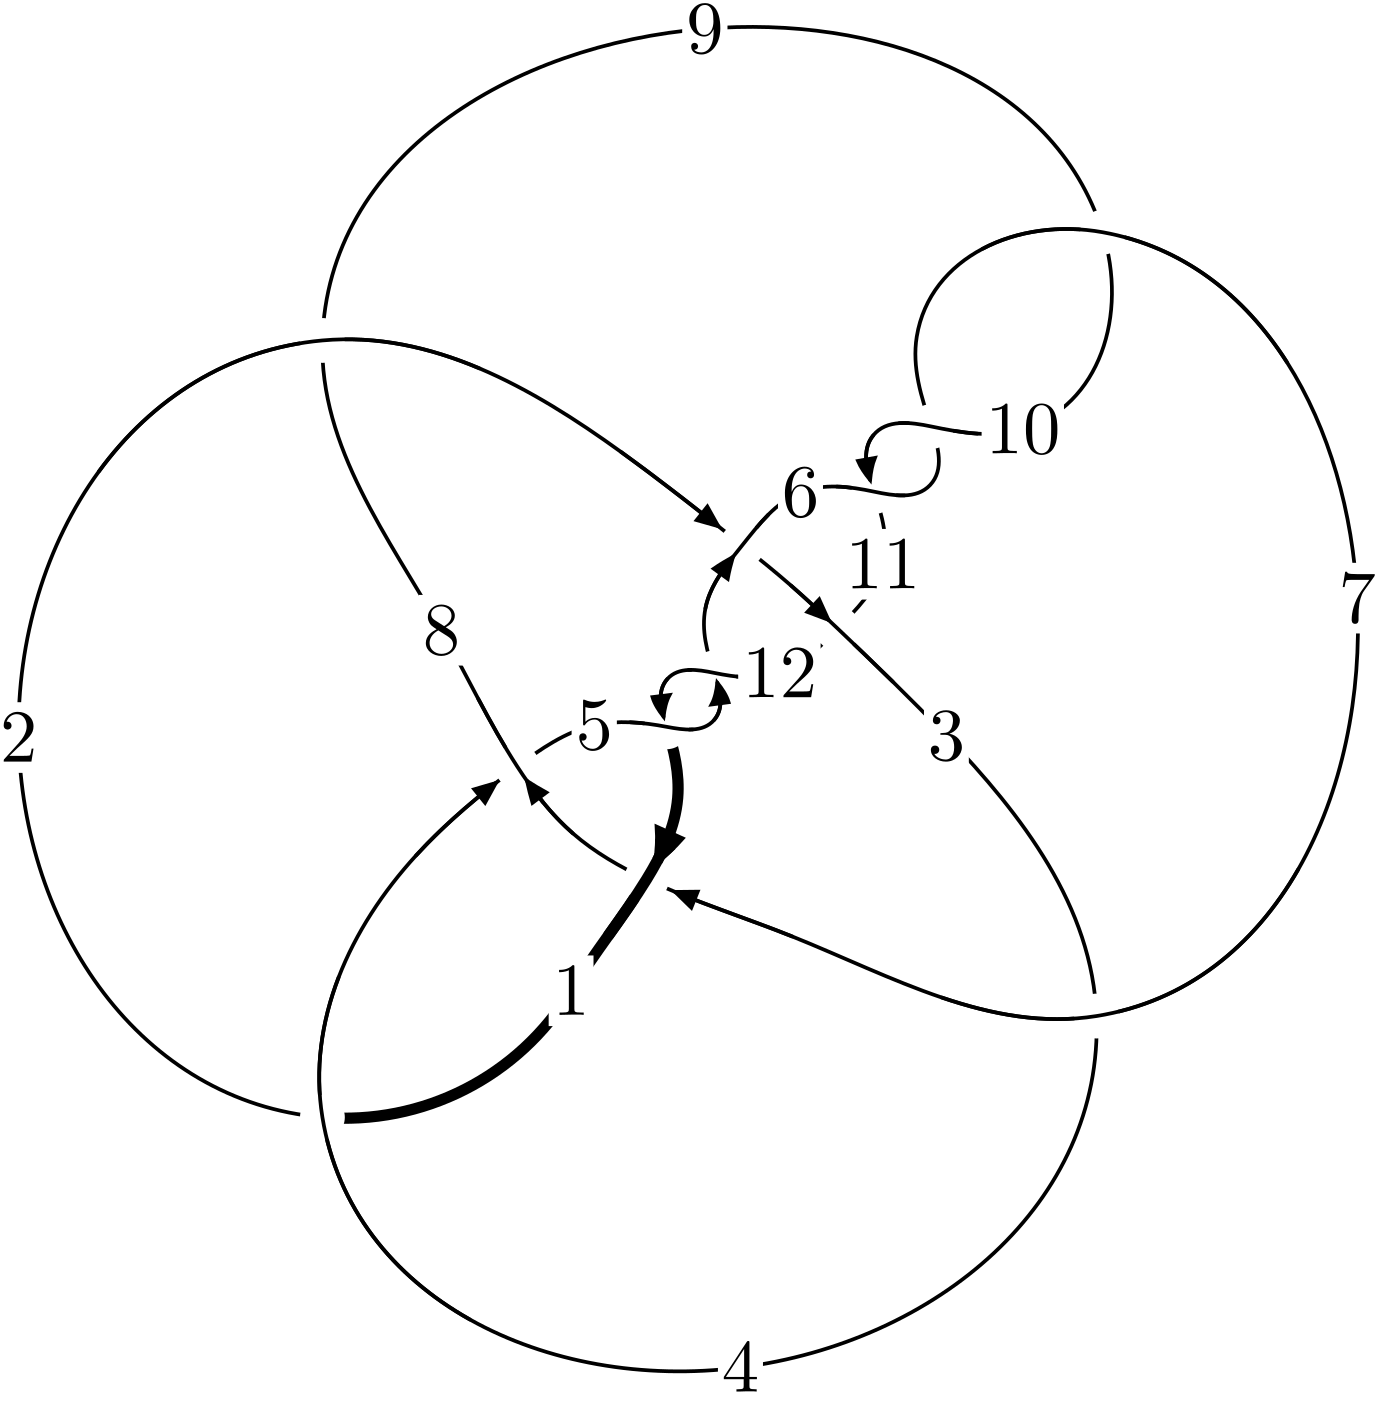
\includegraphics[width=112pt]{../../../GIT/diagram.site/Diagrams/png/2835_12n_0746.png}\\
\ \ \ A knot diagram\footnotemark}&
\allowdisplaybreaks
\textbf{Linearized knot diagam} \\
\cline{2-2}
 &
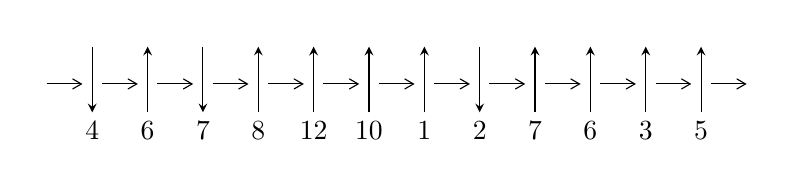
\begin{tikzpicture}[x=20pt, y=17pt]
	% nodes
	\node (C0) at (0, 0) {};
	\node (C1) at (1, 0) {};
	\node (C1U) at (1, +1) {};
	\node (C1D) at (1, -1) {4};

	\node (C2) at (2, 0) {};
	\node (C2U) at (2, +1) {};
	\node (C2D) at (2, -1) {6};

	\node (C3) at (3, 0) {};
	\node (C3U) at (3, +1) {};
	\node (C3D) at (3, -1) {7};

	\node (C4) at (4, 0) {};
	\node (C4U) at (4, +1) {};
	\node (C4D) at (4, -1) {8};

	\node (C5) at (5, 0) {};
	\node (C5U) at (5, +1) {};
	\node (C5D) at (5, -1) {12};

	\node (C6) at (6, 0) {};
	\node (C6U) at (6, +1) {};
	\node (C6D) at (6, -1) {10};

	\node (C7) at (7, 0) {};
	\node (C7U) at (7, +1) {};
	\node (C7D) at (7, -1) {1};

	\node (C8) at (8, 0) {};
	\node (C8U) at (8, +1) {};
	\node (C8D) at (8, -1) {2};

	\node (C9) at (9, 0) {};
	\node (C9U) at (9, +1) {};
	\node (C9D) at (9, -1) {7};

	\node (C10) at (10, 0) {};
	\node (C10U) at (10, +1) {};
	\node (C10D) at (10, -1) {6};

	\node (C11) at (11, 0) {};
	\node (C11U) at (11, +1) {};
	\node (C11D) at (11, -1) {3};

	\node (C12) at (12, 0) {};
	\node (C12U) at (12, +1) {};
	\node (C12D) at (12, -1) {5};
	\node (C13) at (13, 0) {};

	% arrows
	\draw[->,>={angle 60}]
	(C0) edge (C1) (C1) edge (C2) (C2) edge (C3) (C3) edge (C4) (C4) edge (C5) (C5) edge (C6) (C6) edge (C7) (C7) edge (C8) (C8) edge (C9) (C9) edge (C10) (C10) edge (C11) (C11) edge (C12) (C12) edge (C13) ;	\draw[->,>=stealth]
	(C1U) edge (C1D) (C2D) edge (C2U) (C3U) edge (C3D) (C4D) edge (C4U) (C5D) edge (C5U) (C6D) edge (C6U) (C7D) edge (C7U) (C8U) edge (C8D) (C9D) edge (C9U) (C10D) edge (C10U) (C11D) edge (C11U) (C12D) edge (C12U) ;
	\end{tikzpicture} \\
\hhline{~~} \\& 
\textbf{Solving Sequence} \\ \cline{2-2} 
 &
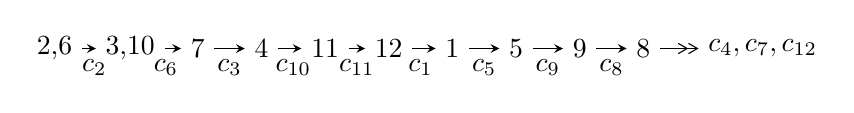
\begin{tikzpicture}[x=23pt, y=7pt]
	% node
	\node (A0) at (-1/8, 0) {2,6};
	\node (A1) at (17/16, 0) {3,10};
	\node (A2) at (17/8, 0) {7};
	\node (A3) at (25/8, 0) {4};
	\node (A4) at (33/8, 0) {11};
	\node (A5) at (41/8, 0) {12};
	\node (A6) at (49/8, 0) {1};
	\node (A7) at (57/8, 0) {5};
	\node (A8) at (65/8, 0) {9};
	\node (A9) at (73/8, 0) {8};
	\node (C1) at (1/2, -1) {$c_{2}$};
	\node (C2) at (13/8, -1) {$c_{6}$};
	\node (C3) at (21/8, -1) {$c_{3}$};
	\node (C4) at (29/8, -1) {$c_{10}$};
	\node (C5) at (37/8, -1) {$c_{11}$};
	\node (C6) at (45/8, -1) {$c_{1}$};
	\node (C7) at (53/8, -1) {$c_{5}$};
	\node (C8) at (61/8, -1) {$c_{9}$};
	\node (C9) at (69/8, -1) {$c_{8}$};
	\node (A10) at (11, 0) {$c_{4},c_{7},c_{12}$};

	% edge
	\draw[->,>=stealth]	
	(A0) edge (A1) (A1) edge (A2) (A2) edge (A3) (A3) edge (A4) (A4) edge (A5) (A5) edge (A6) (A6) edge (A7) (A7) edge (A8) (A8) edge (A9) ;
	\draw[->>,>={angle 60}]	
	(A9) edge (A10);
\end{tikzpicture} \\ 

\end{tabular} \\

\footnotetext{
The image of knot diagram is generated by the software ``\textbf{Draw programme}" developed by Andrew Bartholomew(\url{http://www.layer8.co.uk/maths/draw/index.htm\#Running-draw}), where we modified some parts for our purpose(\url{https://github.com/CATsTAILs/LinksPainter}).
}\phantom \\ \newline 
\centering \textbf{Ideals for irreducible components\footnotemark of $X_{\text{par}}$} 
 
\begin{align*}
I^u_{1}&=\langle 
b- u,\;-1.83924\times10^{21} u^{27}+7.51768\times10^{21} u^{26}+\cdots+3.02460\times10^{21} a-9.01849\times10^{21},\\
\phantom{I^u_{1}}&\phantom{= \langle  }u^{28}-2 u^{27}+\cdots-2 u+1\rangle \\
I^u_{2}&=\langle 
-4.38637\times10^{21} u^{23}-6.05223\times10^{21} u^{22}+\cdots+9.74526\times10^{20} b+2.66742\times10^{23},\\
\phantom{I^u_{2}}&\phantom{= \langle  }-1.58823\times10^{23} u^{23}-2.15936\times10^{23} u^{22}+\cdots+2.24141\times10^{22} a+9.91766\times10^{24},\\
\phantom{I^u_{2}}&\phantom{= \langle  }u^{24}+u^{23}+\cdots-230 u+23\rangle \\
I^u_{3}&=\langle 
b+u,\;-99658301453 u^{19}+22815726133 u^{18}+\cdots+73658938123 a-286826314291,\\
\phantom{I^u_{3}}&\phantom{= \langle  }u^{20}- u^{19}+\cdots-2 u+1\rangle \\
I^u_{4}&=\langle 
-3.66729\times10^{26} u^{23}+3.10786\times10^{26} u^{22}+\cdots+9.53312\times10^{27} b-4.94358\times10^{28},\\
\phantom{I^u_{4}}&\phantom{= \langle  }-7.82120\times10^{27} u^{23}+8.56311\times10^{27} u^{22}+\cdots+4.09924\times10^{29} a-2.28465\times10^{30},\\
\phantom{I^u_{4}}&\phantom{= \langle  }u^{24}-8 u^{22}+\cdots+242 u+43\rangle \\
I^u_{5}&=\langle 
b- u,\;a,\;u^3+u^2-1\rangle \\
\\
\end{align*}
\raggedright * 5 irreducible components of $\dim_{\mathbb{C}}=0$, with total 99 representations.\\
\footnotetext{All coefficients of polynomials are rational numbers. But the coefficients are sometimes approximated in decimal forms when there is not enough margin.}
\newpage
\renewcommand{\arraystretch}{1}
\centering \section*{I. $I^u_{1}= \langle b- u,\;-1.84\times10^{21} u^{27}+7.52\times10^{21} u^{26}+\cdots+3.02\times10^{21} a-9.02\times10^{21},\;u^{28}-2 u^{27}+\cdots-2 u+1 \rangle$}
\flushleft \textbf{(i) Arc colorings}\\
\begin{tabular}{m{7pt} m{180pt} m{7pt} m{180pt} }
\flushright $a_{2}=$&$\begin{pmatrix}1\\0\end{pmatrix}$ \\
\flushright $a_{6}=$&$\begin{pmatrix}0\\u\end{pmatrix}$ \\
\flushright $a_{3}=$&$\begin{pmatrix}1\\- u^2\end{pmatrix}$ \\
\flushright $a_{10}=$&$\begin{pmatrix}0.608092 u^{27}-2.48551 u^{26}+\cdots-16.5137 u+2.98171\\u\end{pmatrix}$ \\
\flushright $a_{7}=$&$\begin{pmatrix}3.02147 u^{27}-5.56752 u^{26}+\cdots-8.71227 u-7.54372\\0.146622 u^{27}-0.672339 u^{26}+\cdots-2.14675 u+1.26933\end{pmatrix}$ \\
\flushright $a_{4}=$&$\begin{pmatrix}1.25423 u^{27}-2.25494 u^{26}+\cdots+7.72816 u+4.89956\\-0.309280 u^{27}+0.794974 u^{26}+\cdots+1.07232 u-0.906326\end{pmatrix}$ \\
\flushright $a_{11}=$&$\begin{pmatrix}0.608092 u^{27}-2.48551 u^{26}+\cdots-16.5137 u+2.98171\\-0.146622 u^{27}+0.672339 u^{26}+\cdots+4.14675 u-1.26933\end{pmatrix}$ \\
\flushright $a_{12}=$&$\begin{pmatrix}0.608092 u^{27}-2.48551 u^{26}+\cdots-15.5137 u+2.98171\\-0.146622 u^{27}+0.672339 u^{26}+\cdots+4.14675 u-1.26933\end{pmatrix}$ \\
\flushright $a_{1}=$&$\begin{pmatrix}2.64646 u^{27}-4.80020 u^{26}+\cdots+5.40118 u-0.731153\\-0.452414 u^{27}+1.16215 u^{26}+\cdots+1.92755 u-0.493859\end{pmatrix}$ \\
\flushright $a_{5}=$&$\begin{pmatrix}-3.31472 u^{27}+6.91219 u^{26}+\cdots+15.0058 u+5.00506\\-0.0676430 u^{27}+0.0431589 u^{26}+\cdots+0.266521 u-0.986574\end{pmatrix}$ \\
\flushright $a_{9}=$&$\begin{pmatrix}2.27197 u^{27}-3.48515 u^{26}+\cdots+13.3274 u-0.442136\\0.317299 u^{27}-0.919860 u^{26}+\cdots-4.21736 u+0.793896\end{pmatrix}$ \\
\flushright $a_{8}=$&$\begin{pmatrix}2.58927 u^{27}-4.40501 u^{26}+\cdots+9.11008 u+0.351760\\0.317299 u^{27}-0.919860 u^{26}+\cdots-4.21736 u+0.793896\end{pmatrix}$\\&\end{tabular}
\flushleft \textbf{(ii) Obstruction class $= -1$}\\~\\
\flushleft \textbf{(iii) Cusp Shapes $= \frac{582961495882437832970}{3024598968157486859593} u^{27}-\frac{7584312197379865856979}{3024598968157486859593} u^{26}+\cdots-\frac{48717383677932330753372}{3024598968157486859593} u+\frac{53712721057335359768630}{3024598968157486859593}$}\\~\\
\newpage\renewcommand{\arraystretch}{1}
\flushleft \textbf{(iv) u-Polynomials at the component}\newline \\
\begin{tabular}{m{50pt}|m{274pt}}
Crossings & \hspace{64pt}u-Polynomials at each crossing \\
\hline $$\begin{aligned}c_{1}\end{aligned}$$&$\begin{aligned}
&u^{28}-21 u^{27}+\cdots-1076 u+85
\end{aligned}$\\
\hline $$\begin{aligned}c_{2},c_{11}\end{aligned}$$&$\begin{aligned}
&u^{28}-2 u^{27}+\cdots-2 u+1
\end{aligned}$\\
\hline $$\begin{aligned}c_{3},c_{8}\end{aligned}$$&$\begin{aligned}
&u^{28}+u^{26}+\cdots+5 u+1
\end{aligned}$\\
\hline $$\begin{aligned}c_{4},c_{7}\end{aligned}$$&$\begin{aligned}
&u^{28}- u^{27}+\cdots- u+1
\end{aligned}$\\
\hline $$\begin{aligned}c_{5},c_{12}\end{aligned}$$&$\begin{aligned}
&u^{28}-16 u^{27}+\cdots-3584 u+256
\end{aligned}$\\
\hline $$\begin{aligned}c_{6},c_{9},c_{10}\end{aligned}$$&$\begin{aligned}
&u^{28}+14 u^{27}+\cdots+388 u+85
\end{aligned}$\\
\hline
\end{tabular}\\~\\
\newpage\renewcommand{\arraystretch}{1}
\flushleft \textbf{(v) Riley Polynomials at the component}\newline \\
\begin{tabular}{m{50pt}|m{274pt}}
Crossings & \hspace{64pt}Riley Polynomials at each crossing \\
\hline $$\begin{aligned}c_{1}\end{aligned}$$&$\begin{aligned}
&y^{28}+5 y^{27}+\cdots+88494 y+7225
\end{aligned}$\\
\hline $$\begin{aligned}c_{2},c_{11}\end{aligned}$$&$\begin{aligned}
&y^{28}-30 y^{27}+\cdots-14 y+1
\end{aligned}$\\
\hline $$\begin{aligned}c_{3},c_{8}\end{aligned}$$&$\begin{aligned}
&y^{28}+2 y^{27}+\cdots- y+1
\end{aligned}$\\
\hline $$\begin{aligned}c_{4},c_{7}\end{aligned}$$&$\begin{aligned}
&y^{28}+5 y^{27}+\cdots+y+1
\end{aligned}$\\
\hline $$\begin{aligned}c_{5},c_{12}\end{aligned}$$&$\begin{aligned}
&y^{28}+24 y^{27}+\cdots-65536 y+65536
\end{aligned}$\\
\hline $$\begin{aligned}c_{6},c_{9},c_{10}\end{aligned}$$&$\begin{aligned}
&y^{28}+14 y^{27}+\cdots-10634 y+7225
\end{aligned}$\\
\hline
\end{tabular}\\~\\
\newpage\flushleft \textbf{(vi) Complex Volumes and Cusp Shapes}
$$\begin{array}{c|c|c}  
\text{Solutions to }I^u_{1}& \I (\text{vol} + \sqrt{-1}CS) & \text{Cusp shape}\\
 \hline 
\begin{aligned}
u &= -1.086820 + 0.335626 I \\
a &= \phantom{-}0.377913 + 0.742585 I \\
b &= -1.086820 + 0.335626 I\end{aligned}
 & -2.65449 - 3.26122 I & \phantom{-}2.78730 + 2.85719 I \\ \hline\begin{aligned}
u &= -1.086820 - 0.335626 I \\
a &= \phantom{-}0.377913 - 0.742585 I \\
b &= -1.086820 - 0.335626 I\end{aligned}
 & -2.65449 + 3.26122 I & \phantom{-}2.78730 - 2.85719 I \\ \hline\begin{aligned}
u &= \phantom{-}1.291560 + 0.285093 I \\
a &= -0.764348 + 0.803904 I \\
b &= \phantom{-}1.291560 + 0.285093 I\end{aligned}
 & -1.20504 + 9.37586 I & \phantom{-}5.06931 - 5.78305 I \\ \hline\begin{aligned}
u &= \phantom{-}1.291560 - 0.285093 I \\
a &= -0.764348 - 0.803904 I \\
b &= \phantom{-}1.291560 - 0.285093 I\end{aligned}
 & -1.20504 - 9.37586 I & \phantom{-}5.06931 + 5.78305 I \\ \hline\begin{aligned}
u &= -0.521856 + 0.406646 I \\
a &= -1.15897 + 1.81439 I \\
b &= -0.521856 + 0.406646 I\end{aligned}
 & -8.79310 - 0.90672 I & \phantom{-}1.94268 + 8.40913 I \\ \hline\begin{aligned}
u &= -0.521856 - 0.406646 I \\
a &= -1.15897 - 1.81439 I \\
b &= -0.521856 - 0.406646 I\end{aligned}
 & -8.79310 + 0.90672 I & \phantom{-}1.94268 - 8.40913 I \\ \hline\begin{aligned}
u &= \phantom{-}1.361260 + 0.077580 I \\
a &= -0.583212 - 0.841707 I \\
b &= \phantom{-}1.361260 + 0.077580 I\end{aligned}
 & \phantom{-}2.74957 + 4.57356 I & \phantom{-}4.51737 - 9.50673 I \\ \hline\begin{aligned}
u &= \phantom{-}1.361260 - 0.077580 I \\
a &= -0.583212 + 0.841707 I \\
b &= \phantom{-}1.361260 - 0.077580 I\end{aligned}
 & \phantom{-}2.74957 - 4.57356 I & \phantom{-}4.51737 + 9.50673 I \\ \hline\begin{aligned}
u &= -1.43638 + 0.07970 I \\
a &= \phantom{-}0.790538 - 0.457604 I \\
b &= -1.43638 + 0.07970 I\end{aligned}
 & \phantom{-}5.39731 + 4.50866 I & \phantom{-}8.58445 - 4.27811 I \\ \hline\begin{aligned}
u &= -1.43638 - 0.07970 I \\
a &= \phantom{-}0.790538 + 0.457604 I \\
b &= -1.43638 - 0.07970 I\end{aligned}
 & \phantom{-}5.39731 - 4.50866 I & \phantom{-}8.58445 + 4.27811 I\\
 \hline 
 \end{array}$$\newpage$$\begin{array}{c|c|c}  
\text{Solutions to }I^u_{1}& \I (\text{vol} + \sqrt{-1}CS) & \text{Cusp shape}\\
 \hline 
\begin{aligned}
u &= -0.537196 + 0.036679 I \\
a &= -0.23574 + 1.76134 I \\
b &= -0.537196 + 0.036679 I\end{aligned}
 & -2.45068 - 2.83732 I & \phantom{-}4.31985 + 3.27002 I \\ \hline\begin{aligned}
u &= -0.537196 - 0.036679 I \\
a &= -0.23574 - 1.76134 I \\
b &= -0.537196 - 0.036679 I\end{aligned}
 & -2.45068 + 2.83732 I & \phantom{-}4.31985 - 3.27002 I \\ \hline\begin{aligned}
u &= -0.071489 + 0.529570 I \\
a &= \phantom{-}1.14088 - 0.95443 I \\
b &= -0.071489 + 0.529570 I\end{aligned}
 & -0.26010 + 1.93004 I & \phantom{-}3.61653 - 5.71528 I \\ \hline\begin{aligned}
u &= -0.071489 - 0.529570 I \\
a &= \phantom{-}1.14088 + 0.95443 I \\
b &= -0.071489 - 0.529570 I\end{aligned}
 & -0.26010 - 1.93004 I & \phantom{-}3.61653 + 5.71528 I \\ \hline\begin{aligned}
u &= \phantom{-}1.43308 + 0.34927 I \\
a &= -0.591407 - 0.524106 I \\
b &= \phantom{-}1.43308 + 0.34927 I\end{aligned}
 & \phantom{-}1.87639 + 2.56909 I & -2.67930 + 1.43996 I \\ \hline\begin{aligned}
u &= \phantom{-}1.43308 - 0.34927 I \\
a &= -0.591407 + 0.524106 I \\
b &= \phantom{-}1.43308 - 0.34927 I\end{aligned}
 & \phantom{-}1.87639 - 2.56909 I & -2.67930 - 1.43996 I \\ \hline\begin{aligned}
u &= \phantom{-}0.282745 + 0.391125 I \\
a &= \phantom{-}0.483464 - 0.962937 I \\
b &= \phantom{-}0.282745 + 0.391125 I\end{aligned}
 & \phantom{-}1.155910 + 0.293260 I & \phantom{-}10.43664 - 2.43272 I \\ \hline\begin{aligned}
u &= \phantom{-}0.282745 - 0.391125 I \\
a &= \phantom{-}0.483464 + 0.962937 I \\
b &= \phantom{-}0.282745 - 0.391125 I\end{aligned}
 & \phantom{-}1.155910 - 0.293260 I & \phantom{-}10.43664 + 2.43272 I \\ \hline\begin{aligned}
u &= \phantom{-}1.42876 + 0.51566 I \\
a &= -0.703819 - 0.195243 I \\
b &= \phantom{-}1.42876 + 0.51566 I\end{aligned}
 & \phantom{-}4.50289 + 1.59330 I & \phantom{-}8.77713 + 1.98299 I \\ \hline\begin{aligned}
u &= \phantom{-}1.42876 - 0.51566 I \\
a &= -0.703819 + 0.195243 I \\
b &= \phantom{-}1.42876 - 0.51566 I\end{aligned}
 & \phantom{-}4.50289 - 1.59330 I & \phantom{-}8.77713 - 1.98299 I\\
 \hline 
 \end{array}$$\newpage$$\begin{array}{c|c|c}  
\text{Solutions to }I^u_{1}& \I (\text{vol} + \sqrt{-1}CS) & \text{Cusp shape}\\
 \hline 
\begin{aligned}
u &= -1.50305 + 0.53936 I \\
a &= \phantom{-}0.767624 - 0.498981 I \\
b &= -1.50305 + 0.53936 I\end{aligned}
 & \phantom{-}3.99815 - 11.69660 I & \phantom{-}6.00000 + 8.56335 I \\ \hline\begin{aligned}
u &= -1.50305 - 0.53936 I \\
a &= \phantom{-}0.767624 + 0.498981 I \\
b &= -1.50305 - 0.53936 I\end{aligned}
 & \phantom{-}3.99815 + 11.69660 I & \phantom{-}6.00000 - 8.56335 I \\ \hline\begin{aligned}
u &= \phantom{-}0.308666 + 0.171864 I \\
a &= -2.41196 - 4.47005 I \\
b &= \phantom{-}0.308666 + 0.171864 I\end{aligned}
 & -11.73900 - 4.61344 I & \phantom{-}11.46925 - 5.36985 I \\ \hline\begin{aligned}
u &= \phantom{-}0.308666 - 0.171864 I \\
a &= -2.41196 + 4.47005 I \\
b &= \phantom{-}0.308666 - 0.171864 I\end{aligned}
 & -11.73900 + 4.61344 I & \phantom{-}11.46925 + 5.36985 I \\ \hline\begin{aligned}
u &= -1.43159 + 0.87843 I \\
a &= \phantom{-}0.704219 - 0.264488 I \\
b &= -1.43159 + 0.87843 I\end{aligned}
 & -3.41771 - 8.95629 I & \phantom{-0.000000 -}0. + 7.40222 I \\ \hline\begin{aligned}
u &= -1.43159 - 0.87843 I \\
a &= \phantom{-}0.704219 + 0.264488 I \\
b &= -1.43159 - 0.87843 I\end{aligned}
 & -3.41771 + 8.95629 I & \phantom{-0.000000 } 0. - 7.40222 I \\ \hline\begin{aligned}
u &= \phantom{-}1.48231 + 0.90624 I \\
a &= -0.815172 - 0.278277 I \\
b &= \phantom{-}1.48231 + 0.90624 I\end{aligned}
 & -2.3195 + 17.0944 I & \phantom{-}6.00000 - 8.92147 I \\ \hline\begin{aligned}
u &= \phantom{-}1.48231 - 0.90624 I \\
a &= -0.815172 + 0.278277 I \\
b &= \phantom{-}1.48231 - 0.90624 I\end{aligned}
 & -2.3195 - 17.0944 I & \phantom{-}6.00000 + 8.92147 I\\
 \hline 
 \end{array}$$\newpage\newpage\renewcommand{\arraystretch}{1}
\centering \section*{II. $I^u_{2}= \langle -4.39\times10^{21} u^{23}-6.05\times10^{21} u^{22}+\cdots+9.75\times10^{20} b+2.67\times10^{23},\;-1.59\times10^{23} u^{23}-2.16\times10^{23} u^{22}+\cdots+2.24\times10^{22} a+9.92\times10^{24},\;u^{24}+u^{23}+\cdots-230 u+23 \rangle$}
\flushleft \textbf{(i) Arc colorings}\\
\begin{tabular}{m{7pt} m{180pt} m{7pt} m{180pt} }
\flushright $a_{2}=$&$\begin{pmatrix}1\\0\end{pmatrix}$ \\
\flushright $a_{6}=$&$\begin{pmatrix}0\\u\end{pmatrix}$ \\
\flushright $a_{3}=$&$\begin{pmatrix}1\\- u^2\end{pmatrix}$ \\
\flushright $a_{10}=$&$\begin{pmatrix}7.08586 u^{23}+9.63395 u^{22}+\cdots+3246.32 u-442.474\\4.50103 u^{23}+6.21044 u^{22}+\cdots+2010.44 u-273.715\end{pmatrix}$ \\
\flushright $a_{7}=$&$\begin{pmatrix}-6.11064 u^{23}-8.32729 u^{22}+\cdots-2798.51 u+378.851\\-0.415380 u^{23}-0.860716 u^{22}+\cdots+46.1813 u-25.3055\end{pmatrix}$ \\
\flushright $a_{4}=$&$\begin{pmatrix}3.27955 u^{23}+4.32985 u^{22}+\cdots+1628.19 u-235.525\\5.50322 u^{23}+7.44656 u^{22}+\cdots+2558.40 u-349.287\end{pmatrix}$ \\
\flushright $a_{11}=$&$\begin{pmatrix}7.08586 u^{23}+9.63395 u^{22}+\cdots+3246.32 u-442.474\\3.60153 u^{23}+5.01071 u^{22}+\cdots+1587.36 u-215.109\end{pmatrix}$ \\
\flushright $a_{12}=$&$\begin{pmatrix}11.5869 u^{23}+15.8444 u^{22}+\cdots+5256.76 u-716.189\\2.94846 u^{23}+4.11075 u^{22}+\cdots+1297.72 u-175.792\end{pmatrix}$ \\
\flushright $a_{1}=$&$\begin{pmatrix}-8.69992 u^{23}-11.2039 u^{22}+\cdots-4497.49 u+658.430\\-10.2679 u^{23}-13.8814 u^{22}+\cdots-4772.27 u+653.807\end{pmatrix}$ \\
\flushright $a_{5}=$&$\begin{pmatrix}2.84349 u^{23}+4.59701 u^{22}+\cdots+726.192 u-47.7595\\-4.55216 u^{23}-5.85791 u^{22}+\cdots-2364.05 u+346.117\end{pmatrix}$ \\
\flushright $a_{9}=$&$\begin{pmatrix}9.11922 u^{23}+12.4058 u^{22}+\cdots+4166.18 u-565.621\\3.66715 u^{23}+5.27000 u^{22}+\cdots+1460.26 u-183.205\end{pmatrix}$ \\
\flushright $a_{8}=$&$\begin{pmatrix}12.7864 u^{23}+17.6758 u^{22}+\cdots+5626.44 u-748.827\\3.66715 u^{23}+5.27000 u^{22}+\cdots+1460.26 u-183.205\end{pmatrix}$\\&\end{tabular}
\flushleft \textbf{(ii) Obstruction class $= -1$}\\~\\
\flushleft \textbf{(iii) Cusp Shapes $= \frac{5311543016724665509336}{88593237130145253275} u^{23}+\frac{7107141086263947951916}{88593237130145253275} u^{22}+\cdots+\frac{506145016549541819876372}{17718647426029050655} u-\frac{351874446634871455526646}{88593237130145253275}$}\\~\\
\newpage\renewcommand{\arraystretch}{1}
\flushleft \textbf{(iv) u-Polynomials at the component}\newline \\
\begin{tabular}{m{50pt}|m{274pt}}
Crossings & \hspace{64pt}u-Polynomials at each crossing \\
\hline $$\begin{aligned}c_{1}\end{aligned}$$&$\begin{aligned}
&(u^4+u^3+u^2- u+1)^6
\end{aligned}$\\
\hline $$\begin{aligned}c_{2},c_{11}\end{aligned}$$&$\begin{aligned}
&u^{24}+u^{23}+\cdots-230 u+23
\end{aligned}$\\
\hline $$\begin{aligned}c_{3},c_{8}\end{aligned}$$&$\begin{aligned}
&u^{24}-2 u^{23}+\cdots+222 u+59
\end{aligned}$\\
\hline $$\begin{aligned}c_{4},c_{7}\end{aligned}$$&$\begin{aligned}
&u^{24}- u^{23}+\cdots+30 u+25
\end{aligned}$\\
\hline $$\begin{aligned}c_{5},c_{12}\end{aligned}$$&$\begin{aligned}
&(u^3+u^2+2 u+1)^8
\end{aligned}$\\
\hline $$\begin{aligned}c_{6},c_{9},c_{10}\end{aligned}$$&$\begin{aligned}
&(u^4- u^3+u^2+u+1)^6
\end{aligned}$\\
\hline
\end{tabular}\\~\\
\newpage\renewcommand{\arraystretch}{1}
\flushleft \textbf{(v) Riley Polynomials at the component}\newline \\
\begin{tabular}{m{50pt}|m{274pt}}
Crossings & \hspace{64pt}Riley Polynomials at each crossing \\
\hline $$\begin{aligned}c_{1},c_{6},c_{9}\\c_{10}\end{aligned}$$&$\begin{aligned}
&(y^4+y^3+5 y^2+y+1)^6
\end{aligned}$\\
\hline $$\begin{aligned}c_{2},c_{11}\end{aligned}$$&$\begin{aligned}
&y^{24}-5 y^{23}+\cdots-17894 y+529
\end{aligned}$\\
\hline $$\begin{aligned}c_{3},c_{8}\end{aligned}$$&$\begin{aligned}
&y^{24}-4 y^{23}+\cdots+71902 y+3481
\end{aligned}$\\
\hline $$\begin{aligned}c_{4},c_{7}\end{aligned}$$&$\begin{aligned}
&y^{24}+7 y^{23}+\cdots+8450 y+625
\end{aligned}$\\
\hline $$\begin{aligned}c_{5},c_{12}\end{aligned}$$&$\begin{aligned}
&(y^3+3 y^2+2 y-1)^8
\end{aligned}$\\
\hline
\end{tabular}\\~\\
\newpage\flushleft \textbf{(vi) Complex Volumes and Cusp Shapes}
$$\begin{array}{c|c|c}  
\text{Solutions to }I^u_{2}& \I (\text{vol} + \sqrt{-1}CS) & \text{Cusp shape}\\
 \hline 
\begin{aligned}
u &= \phantom{-}0.871397 + 0.215536 I \\
a &= \phantom{-}0.70645 - 1.47436 I \\
b &= -1.288690 + 0.118319 I\end{aligned}
 & -0.78305 - 1.85791 I & \phantom{-}3.78084 + 7.29993 I \\ \hline\begin{aligned}
u &= \phantom{-}0.871397 - 0.215536 I \\
a &= \phantom{-}0.70645 + 1.47436 I \\
b &= -1.288690 - 0.118319 I\end{aligned}
 & -0.78305 + 1.85791 I & \phantom{-}3.78084 - 7.29993 I \\ \hline\begin{aligned}
u &= -0.481220 + 1.117750 I \\
a &= \phantom{-}0.537698 + 0.156233 I \\
b &= -1.45439 + 0.43085 I\end{aligned}
 & -5.26521 - 1.85791 I & \phantom{-}1.19965 + 7.29993 I \\ \hline\begin{aligned}
u &= -0.481220 - 1.117750 I \\
a &= \phantom{-}0.537698 - 0.156233 I \\
b &= -1.45439 - 0.43085 I\end{aligned}
 & -5.26521 + 1.85791 I & \phantom{-}1.19965 - 7.29993 I \\ \hline\begin{aligned}
u &= -1.259050 + 0.270524 I \\
a &= -0.893362 + 0.707527 I \\
b &= \phantom{-}1.32599 - 0.61457 I\end{aligned}
 & \phantom{-}3.35454 - 4.68603 I & \phantom{-}10.3101 + 10.2794 I \\ \hline\begin{aligned}
u &= -1.259050 - 0.270524 I \\
a &= -0.893362 - 0.707527 I \\
b &= \phantom{-}1.32599 + 0.61457 I\end{aligned}
 & \phantom{-}3.35454 + 4.68603 I & \phantom{-}10.3101 - 10.2794 I \\ \hline\begin{aligned}
u &= -1.288690 + 0.118319 I \\
a &= -0.798244 + 0.805500 I \\
b &= \phantom{-}0.871397 + 0.215536 I\end{aligned}
 & -0.78305 - 1.85791 I & \phantom{-}3.78084 + 7.29993 I \\ \hline\begin{aligned}
u &= -1.288690 - 0.118319 I \\
a &= -0.798244 - 0.805500 I \\
b &= \phantom{-}0.871397 - 0.215536 I\end{aligned}
 & -0.78305 + 1.85791 I & \phantom{-}3.78084 - 7.29993 I \\ \hline\begin{aligned}
u &= \phantom{-}1.32599 + 0.61457 I \\
a &= \phantom{-}0.905290 + 0.434484 I \\
b &= -1.259050 - 0.270524 I\end{aligned}
 & \phantom{-}3.35454 + 4.68603 I & \phantom{-}10.3101 - 10.2794 I \\ \hline\begin{aligned}
u &= \phantom{-}1.32599 - 0.61457 I \\
a &= \phantom{-}0.905290 - 0.434484 I \\
b &= -1.259050 + 0.270524 I\end{aligned}
 & \phantom{-}3.35454 - 4.68603 I & \phantom{-}10.3101 + 10.2794 I\\
 \hline 
 \end{array}$$\newpage$$\begin{array}{c|c|c}  
\text{Solutions to }I^u_{2}& \I (\text{vol} + \sqrt{-1}CS) & \text{Cusp shape}\\
 \hline 
\begin{aligned}
u &= -0.03872 + 1.51471 I \\
a &= -0.339611 + 0.294797 I \\
b &= \phantom{-}0.349222 + 0.081162 I\end{aligned}
 & -1.12763 + 4.68603 I & \phantom{-}7.72892 - 10.27938 I \\ \hline\begin{aligned}
u &= -0.03872 - 1.51471 I \\
a &= -0.339611 - 0.294797 I \\
b &= \phantom{-}0.349222 - 0.081162 I\end{aligned}
 & -1.12763 - 4.68603 I & \phantom{-}7.72892 + 10.27938 I \\ \hline\begin{aligned}
u &= -1.45439 + 0.43085 I \\
a &= \phantom{-}0.372404 - 0.251224 I \\
b &= -0.481220 + 1.117750 I\end{aligned}
 & -5.26521 - 1.85791 I & \phantom{-}1.19965 + 7.29993 I \\ \hline\begin{aligned}
u &= -1.45439 - 0.43085 I \\
a &= \phantom{-}0.372404 + 0.251224 I \\
b &= -0.481220 - 1.117750 I\end{aligned}
 & -5.26521 + 1.85791 I & \phantom{-}1.19965 - 7.29993 I \\ \hline\begin{aligned}
u &= \phantom{-}1.49772 + 0.63712 I \\
a &= \phantom{-}0.800074 + 0.415791 I \\
b &= -1.23605 - 1.10308 I\end{aligned}
 & -0.78305 + 7.51416 I & \phantom{-}3.78084 - 13.25883 I \\ \hline\begin{aligned}
u &= \phantom{-}1.49772 - 0.63712 I \\
a &= \phantom{-}0.800074 - 0.415791 I \\
b &= -1.23605 + 1.10308 I\end{aligned}
 & -0.78305 - 7.51416 I & \phantom{-}3.78084 + 13.25883 I \\ \hline\begin{aligned}
u &= \phantom{-}0.349222 + 0.081162 I \\
a &= -1.50940 - 1.15491 I \\
b &= -0.03872 + 1.51471 I\end{aligned}
 & -1.12763 + 4.68603 I & \phantom{-}7.72892 - 10.27938 I \\ \hline\begin{aligned}
u &= \phantom{-}0.349222 - 0.081162 I \\
a &= -1.50940 + 1.15491 I \\
b &= -0.03872 - 1.51471 I\end{aligned}
 & -1.12763 - 4.68603 I & \phantom{-}7.72892 + 10.27938 I \\ \hline\begin{aligned}
u &= \phantom{-}0.352036 + 0.040102 I \\
a &= -1.04733 + 1.61298 I \\
b &= \phantom{-}0.86175 + 2.12125 I\end{aligned}
 & -5.26521 - 7.51416 I & \phantom{-}1.19965 + 13.25883 I \\ \hline\begin{aligned}
u &= \phantom{-}0.352036 - 0.040102 I \\
a &= -1.04733 - 1.61298 I \\
b &= \phantom{-}0.86175 - 2.12125 I\end{aligned}
 & -5.26521 + 7.51416 I & \phantom{-}1.19965 - 13.25883 I\\
 \hline 
 \end{array}$$\newpage$$\begin{array}{c|c|c}  
\text{Solutions to }I^u_{2}& \I (\text{vol} + \sqrt{-1}CS) & \text{Cusp shape}\\
 \hline 
\begin{aligned}
u &= -1.23605 + 1.10308 I \\
a &= -0.875509 + 0.134887 I \\
b &= \phantom{-}1.49772 - 0.63712 I\end{aligned}
 & -0.78305 - 7.51416 I & \phantom{-}3.78084 + 13.25883 I \\ \hline\begin{aligned}
u &= -1.23605 - 1.10308 I \\
a &= -0.875509 - 0.134887 I \\
b &= \phantom{-}1.49772 + 0.63712 I\end{aligned}
 & -0.78305 + 7.51416 I & \phantom{-}3.78084 - 13.25883 I \\ \hline\begin{aligned}
u &= \phantom{-}0.86175 + 2.12125 I \\
a &= \phantom{-}0.141530 + 0.261800 I \\
b &= \phantom{-}0.352036 + 0.040102 I\end{aligned}
 & -5.26521 - 7.51416 I & \phantom{-0.000000 } 0 \\ \hline\begin{aligned}
u &= \phantom{-}0.86175 - 2.12125 I \\
a &= \phantom{-}0.141530 - 0.261800 I \\
b &= \phantom{-}0.352036 - 0.040102 I\end{aligned}
 & -5.26521 + 7.51416 I & \phantom{-0.000000 } 0\\
 \hline 
 \end{array}$$\newpage\newpage\renewcommand{\arraystretch}{1}
\centering \section*{III. $I^u_{3}= \langle b+u,\;-9.97\times10^{10} u^{19}+2.28\times10^{10} u^{18}+\cdots+7.37\times10^{10} a-2.87\times10^{11},\;u^{20}- u^{19}+\cdots-2 u+1 \rangle$}
\flushleft \textbf{(i) Arc colorings}\\
\begin{tabular}{m{7pt} m{180pt} m{7pt} m{180pt} }
\flushright $a_{2}=$&$\begin{pmatrix}1\\0\end{pmatrix}$ \\
\flushright $a_{6}=$&$\begin{pmatrix}0\\u\end{pmatrix}$ \\
\flushright $a_{3}=$&$\begin{pmatrix}1\\- u^2\end{pmatrix}$ \\
\flushright $a_{10}=$&$\begin{pmatrix}1.35297 u^{19}-0.309748 u^{18}+\cdots+5.01927 u+3.89398\\- u\end{pmatrix}$ \\
\flushright $a_{7}=$&$\begin{pmatrix}3.05617 u^{19}-3.31440 u^{18}+\cdots+26.4727 u-6.68081\\0.0448430 u^{19}+0.229731 u^{18}+\cdots+0.266527 u+1.04322\end{pmatrix}$ \\
\flushright $a_{4}=$&$\begin{pmatrix}3.73189 u^{19}-2.90830 u^{18}+\cdots+22.5207 u+2.75146\\-0.0798962 u^{19}+0.122919 u^{18}+\cdots-1.56402 u+0.709081\end{pmatrix}$ \\
\flushright $a_{11}=$&$\begin{pmatrix}1.35297 u^{19}-0.309748 u^{18}+\cdots+5.01927 u+3.89398\\0.0448430 u^{19}+0.229731 u^{18}+\cdots-1.73347 u+1.04322\end{pmatrix}$ \\
\flushright $a_{12}=$&$\begin{pmatrix}1.35297 u^{19}-0.309748 u^{18}+\cdots+4.01927 u+3.89398\\0.0448430 u^{19}+0.229731 u^{18}+\cdots-1.73347 u+1.04322\end{pmatrix}$ \\
\flushright $a_{1}=$&$\begin{pmatrix}-2.24854 u^{19}+0.516651 u^{18}+\cdots-4.37312 u-7.02363\\-0.0516704 u^{19}-0.300485 u^{18}+\cdots+2.04578 u-0.397752\end{pmatrix}$ \\
\flushright $a_{5}=$&$\begin{pmatrix}-3.14585 u^{19}+2.85493 u^{18}+\cdots-25.0058 u+4.59437\\-0.124739 u^{19}-0.106813 u^{18}+\cdots-0.830543 u-1.33414\end{pmatrix}$ \\
\flushright $a_{9}=$&$\begin{pmatrix}-2.83500 u^{19}+1.12947 u^{18}+\cdots-12.5781 u-7.07266\\0.266234 u^{19}-0.515357 u^{18}+\cdots+3.30610 u-1.30145\end{pmatrix}$ \\
\flushright $a_{8}=$&$\begin{pmatrix}-2.56877 u^{19}+0.614111 u^{18}+\cdots-9.27198 u-8.37411\\0.266234 u^{19}-0.515357 u^{18}+\cdots+3.30610 u-1.30145\end{pmatrix}$\\&\end{tabular}
\flushleft \textbf{(ii) Obstruction class $= 1$}\\~\\
\flushleft \textbf{(iii) Cusp Shapes $= -\frac{456675119914}{73658938123} u^{19}+\frac{414145420365}{73658938123} u^{18}+\cdots-\frac{3019589803806}{73658938123} u-\frac{62318108709}{73658938123}$}\\~\\
\newpage\renewcommand{\arraystretch}{1}
\flushleft \textbf{(iv) u-Polynomials at the component}\newline \\
\begin{tabular}{m{50pt}|m{274pt}}
Crossings & \hspace{64pt}u-Polynomials at each crossing \\
\hline $$\begin{aligned}c_{1}\end{aligned}$$&$\begin{aligned}
&u^{20}-8 u^{19}+\cdots+3 u^2+1
\end{aligned}$\\
\hline $$\begin{aligned}c_{2},c_{11}\end{aligned}$$&$\begin{aligned}
&u^{20}- u^{19}+\cdots-2 u+1
\end{aligned}$\\
\hline $$\begin{aligned}c_{3},c_{8}\end{aligned}$$&$\begin{aligned}
&u^{20}+u^{19}+\cdots+3 u+13
\end{aligned}$\\
\hline $$\begin{aligned}c_{4},c_{7}\end{aligned}$$&$\begin{aligned}
&u^{20}+4 u^{18}+\cdots- u+1
\end{aligned}$\\
\hline $$\begin{aligned}c_{5}\end{aligned}$$&$\begin{aligned}
&u^{20}+12 u^{18}+\cdots- u+3
\end{aligned}$\\
\hline $$\begin{aligned}c_{6}\end{aligned}$$&$\begin{aligned}
&u^{20}+7 u^{19}+\cdots+7 u^2+1
\end{aligned}$\\
\hline $$\begin{aligned}c_{9},c_{10}\end{aligned}$$&$\begin{aligned}
&u^{20}-7 u^{19}+\cdots+7 u^2+1
\end{aligned}$\\
\hline $$\begin{aligned}c_{12}\end{aligned}$$&$\begin{aligned}
&u^{20}+12 u^{18}+\cdots+u+3
\end{aligned}$\\
\hline
\end{tabular}\\~\\
\newpage\renewcommand{\arraystretch}{1}
\flushleft \textbf{(v) Riley Polynomials at the component}\newline \\
\begin{tabular}{m{50pt}|m{274pt}}
Crossings & \hspace{64pt}Riley Polynomials at each crossing \\
\hline $$\begin{aligned}c_{1}\end{aligned}$$&$\begin{aligned}
&y^{20}+4 y^{19}+\cdots+6 y+1
\end{aligned}$\\
\hline $$\begin{aligned}c_{2},c_{11}\end{aligned}$$&$\begin{aligned}
&y^{20}-7 y^{19}+\cdots+14 y+1
\end{aligned}$\\
\hline $$\begin{aligned}c_{3},c_{8}\end{aligned}$$&$\begin{aligned}
&y^{20}+y^{19}+\cdots-425 y+169
\end{aligned}$\\
\hline $$\begin{aligned}c_{4},c_{7}\end{aligned}$$&$\begin{aligned}
&y^{20}+8 y^{19}+\cdots+5 y+1
\end{aligned}$\\
\hline $$\begin{aligned}c_{5},c_{12}\end{aligned}$$&$\begin{aligned}
&y^{20}+24 y^{19}+\cdots+5 y+9
\end{aligned}$\\
\hline $$\begin{aligned}c_{6},c_{9},c_{10}\end{aligned}$$&$\begin{aligned}
&y^{20}+13 y^{19}+\cdots+14 y+1
\end{aligned}$\\
\hline
\end{tabular}\\~\\
\newpage\flushleft \textbf{(vi) Complex Volumes and Cusp Shapes}
$$\begin{array}{c|c|c}  
\text{Solutions to }I^u_{3}& \I (\text{vol} + \sqrt{-1}CS) & \text{Cusp shape}\\
 \hline 
\begin{aligned}
u &= \phantom{-}0.206860 + 0.912738 I \\
a &= \phantom{-}0.595089 + 0.399266 I \\
b &= -0.206860 - 0.912738 I\end{aligned}
 & -1.87110 - 4.11491 I & -1.55747 + 5.09443 I \\ \hline\begin{aligned}
u &= \phantom{-}0.206860 - 0.912738 I \\
a &= \phantom{-}0.595089 - 0.399266 I \\
b &= -0.206860 + 0.912738 I\end{aligned}
 & -1.87110 + 4.11491 I & -1.55747 - 5.09443 I \\ \hline\begin{aligned}
u &= \phantom{-}1.146640 + 0.158956 I \\
a &= \phantom{-}0.833442 - 0.963122 I \\
b &= -1.146640 - 0.158956 I\end{aligned}
 & -0.308612 - 0.887866 I & \phantom{-}7.01392 + 0.89869 I \\ \hline\begin{aligned}
u &= \phantom{-}1.146640 - 0.158956 I \\
a &= \phantom{-}0.833442 + 0.963122 I \\
b &= -1.146640 + 0.158956 I\end{aligned}
 & -0.308612 + 0.887866 I & \phantom{-}7.01392 - 0.89869 I \\ \hline\begin{aligned}
u &= -0.764508 + 1.012020 I \\
a &= -0.039227 + 0.271965 I \\
b &= \phantom{-}0.764508 - 1.012020 I\end{aligned}
 & -5.47737 + 6.62738 I & -0.42430 - 3.51997 I \\ \hline\begin{aligned}
u &= -0.764508 - 1.012020 I \\
a &= -0.039227 - 0.271965 I \\
b &= \phantom{-}0.764508 + 1.012020 I\end{aligned}
 & -5.47737 - 6.62738 I & -0.42430 + 3.51997 I \\ \hline\begin{aligned}
u &= -0.331623 + 0.638727 I \\
a &= -1.26938 + 0.62846 I \\
b &= \phantom{-}0.331623 - 0.638727 I\end{aligned}
 & -3.79735 - 3.38074 I & -3.18735 + 5.13211 I \\ \hline\begin{aligned}
u &= -0.331623 - 0.638727 I \\
a &= -1.26938 - 0.62846 I \\
b &= \phantom{-}0.331623 + 0.638727 I\end{aligned}
 & -3.79735 + 3.38074 I & -3.18735 - 5.13211 I \\ \hline\begin{aligned}
u &= \phantom{-}0.411689 + 0.583746 I \\
a &= -1.48118 - 1.12864 I \\
b &= -0.411689 - 0.583746 I\end{aligned}
 & -9.13088 + 0.23260 I & -5.20121 + 0.99282 I \\ \hline\begin{aligned}
u &= \phantom{-}0.411689 - 0.583746 I \\
a &= -1.48118 + 1.12864 I \\
b &= -0.411689 + 0.583746 I\end{aligned}
 & -9.13088 - 0.23260 I & -5.20121 - 0.99282 I\\
 \hline 
 \end{array}$$\newpage$$\begin{array}{c|c|c}  
\text{Solutions to }I^u_{3}& \I (\text{vol} + \sqrt{-1}CS) & \text{Cusp shape}\\
 \hline 
\begin{aligned}
u &= -1.277620 + 0.235723 I \\
a &= -0.755026 + 0.731922 I \\
b &= \phantom{-}1.277620 - 0.235723 I\end{aligned}
 & \phantom{-}2.53448 - 3.53693 I & \phantom{-}4.49394 + 2.65444 I \\ \hline\begin{aligned}
u &= -1.277620 - 0.235723 I \\
a &= -0.755026 - 0.731922 I \\
b &= \phantom{-}1.277620 + 0.235723 I\end{aligned}
 & \phantom{-}2.53448 + 3.53693 I & \phantom{-}4.49394 - 2.65444 I \\ \hline\begin{aligned}
u &= \phantom{-}0.896773 + 0.960875 I \\
a &= \phantom{-}0.339283 + 0.184359 I \\
b &= -0.896773 - 0.960875 I\end{aligned}
 & -5.79310 + 1.03199 I & -4.20712 - 0.39355 I \\ \hline\begin{aligned}
u &= \phantom{-}0.896773 - 0.960875 I \\
a &= \phantom{-}0.339283 - 0.184359 I \\
b &= -0.896773 + 0.960875 I\end{aligned}
 & -5.79310 - 1.03199 I & -4.20712 + 0.39355 I \\ \hline\begin{aligned}
u &= -1.259400 + 0.425629 I \\
a &= -0.881755 + 0.330751 I \\
b &= \phantom{-}1.259400 - 0.425629 I\end{aligned}
 & \phantom{-}3.54204 - 2.99255 I & \phantom{-}6.08654 + 3.89052 I \\ \hline\begin{aligned}
u &= -1.259400 - 0.425629 I \\
a &= -0.881755 - 0.330751 I \\
b &= \phantom{-}1.259400 + 0.425629 I\end{aligned}
 & \phantom{-}3.54204 + 2.99255 I & \phantom{-}6.08654 - 3.89052 I \\ \hline\begin{aligned}
u &= \phantom{-}0.095406 + 0.374240 I \\
a &= \phantom{-}4.30822 + 1.24073 I \\
b &= -0.095406 - 0.374240 I\end{aligned}
 & -11.97380 + 4.82580 I & -7.61339 - 11.34574 I \\ \hline\begin{aligned}
u &= \phantom{-}0.095406 - 0.374240 I \\
a &= \phantom{-}4.30822 - 1.24073 I \\
b &= -0.095406 + 0.374240 I\end{aligned}
 & -11.97380 - 4.82580 I & -7.61339 + 11.34574 I \\ \hline\begin{aligned}
u &= \phantom{-}1.37578 + 0.84536 I \\
a &= \phantom{-}0.850537 + 0.232509 I \\
b &= -1.37578 - 0.84536 I\end{aligned}
 & -0.62299 + 6.60843 I & \phantom{-}4.59643 - 3.39212 I \\ \hline\begin{aligned}
u &= \phantom{-}1.37578 - 0.84536 I \\
a &= \phantom{-}0.850537 - 0.232509 I \\
b &= -1.37578 + 0.84536 I\end{aligned}
 & -0.62299 - 6.60843 I & \phantom{-}4.59643 + 3.39212 I\\
 \hline 
 \end{array}$$\newpage\newpage\renewcommand{\arraystretch}{1}
\centering \section*{IV. $I^u_{4}= \langle -3.67\times10^{26} u^{23}+3.11\times10^{26} u^{22}+\cdots+9.53\times10^{27} b-4.94\times10^{28},\;-7.82\times10^{27} u^{23}+8.56\times10^{27} u^{22}+\cdots+4.10\times10^{29} a-2.28\times10^{30},\;u^{24}-8 u^{22}+\cdots+242 u+43 \rangle$}
\flushleft \textbf{(i) Arc colorings}\\
\begin{tabular}{m{7pt} m{180pt} m{7pt} m{180pt} }
\flushright $a_{2}=$&$\begin{pmatrix}1\\0\end{pmatrix}$ \\
\flushright $a_{6}=$&$\begin{pmatrix}0\\u\end{pmatrix}$ \\
\flushright $a_{3}=$&$\begin{pmatrix}1\\- u^2\end{pmatrix}$ \\
\flushright $a_{10}=$&$\begin{pmatrix}0.0190796 u^{23}-0.0208895 u^{22}+\cdots+23.9335 u+5.57336\\0.0384689 u^{23}-0.0326006 u^{22}+\cdots+20.6673 u+5.18569\end{pmatrix}$ \\
\flushright $a_{7}=$&$\begin{pmatrix}-0.0308549 u^{23}-0.0309852 u^{22}+\cdots+13.1028 u+4.24203\\0.00630508 u^{23}+0.0121205 u^{22}+\cdots-4.93815 u+0.374359\end{pmatrix}$ \\
\flushright $a_{4}=$&$\begin{pmatrix}0.00429981 u^{23}+0.00889826 u^{22}+\cdots+1.52545 u+4.03528\\0.0208895 u^{23}+0.0219619 u^{22}+\cdots-0.956087 u+1.82042\end{pmatrix}$ \\
\flushright $a_{11}=$&$\begin{pmatrix}0.0190796 u^{23}-0.0208895 u^{22}+\cdots+23.9335 u+5.57336\\0.0604308 u^{23}-0.0273914 u^{22}+\cdots+16.4324 u+4.28744\end{pmatrix}$ \\
\flushright $a_{12}=$&$\begin{pmatrix}0.0575485 u^{23}-0.0534901 u^{22}+\cdots+44.6007 u+10.7591\\0.0568322 u^{23}-0.00741976 u^{22}+\cdots+10.1972 u+2.88562\end{pmatrix}$ \\
\flushright $a_{1}=$&$\begin{pmatrix}-0.0301588 u^{23}+0.0179193 u^{22}+\cdots-26.1094 u-9.14299\\-0.0107939 u^{23}-0.00843626 u^{22}+\cdots-9.79673 u-3.96761\end{pmatrix}$ \\
\flushright $a_{5}=$&$\begin{pmatrix}0.00413390 u^{23}-0.0355708 u^{22}+\cdots+10.5611 u-4.01184\\-0.0204326 u^{23}-0.0402020 u^{22}+\cdots+10.2954 u-0.924994\end{pmatrix}$ \\
\flushright $a_{9}=$&$\begin{pmatrix}-0.0534723 u^{23}-0.0588566 u^{22}+\cdots+26.2658 u+4.41066\\0.0352500 u^{23}+0.00717673 u^{22}+\cdots+2.95256 u+1.45494\end{pmatrix}$ \\
\flushright $a_{8}=$&$\begin{pmatrix}-0.0182223 u^{23}-0.0516798 u^{22}+\cdots+29.2184 u+5.86560\\0.0352500 u^{23}+0.00717673 u^{22}+\cdots+2.95256 u+1.45494\end{pmatrix}$\\&\end{tabular}
\flushleft \textbf{(ii) Obstruction class $= -1$}\\~\\
\flushleft \textbf{(iii) Cusp Shapes $= -\frac{535804160101971736815030556}{9533118023002544093158027727} u^{23}-\frac{629721383815858353997296608}{9533118023002544093158027727} u^{22}+\cdots+\frac{122994948289871385854632596364}{9533118023002544093158027727} u-\frac{47116154343604428037295209270}{9533118023002544093158027727}$}\\~\\
\newpage\renewcommand{\arraystretch}{1}
\flushleft \textbf{(iv) u-Polynomials at the component}\newline \\
\begin{tabular}{m{50pt}|m{274pt}}
Crossings & \hspace{64pt}u-Polynomials at each crossing \\
\hline $$\begin{aligned}c_{1}\end{aligned}$$&$\begin{aligned}
&(u^4+2 u^3+2 u^2+u+1)^6
\end{aligned}$\\
\hline $$\begin{aligned}c_{2},c_{11}\end{aligned}$$&$\begin{aligned}
&u^{24}-8 u^{22}+\cdots+242 u+43
\end{aligned}$\\
\hline $$\begin{aligned}c_{3},c_{8}\end{aligned}$$&$\begin{aligned}
&u^{24}+u^{23}+\cdots-36 u+19
\end{aligned}$\\
\hline $$\begin{aligned}c_{4},c_{7}\end{aligned}$$&$\begin{aligned}
&u^{24}+4 u^{22}+\cdots+8 u+7
\end{aligned}$\\
\hline $$\begin{aligned}c_{5},c_{12}\end{aligned}$$&$\begin{aligned}
&(u^3+u^2+2 u+1)^8
\end{aligned}$\\
\hline $$\begin{aligned}c_{6},c_{9},c_{10}\end{aligned}$$&$\begin{aligned}
&(u^4-2 u^3+2 u^2- u+1)^6
\end{aligned}$\\
\hline
\end{tabular}\\~\\
\newpage\renewcommand{\arraystretch}{1}
\flushleft \textbf{(v) Riley Polynomials at the component}\newline \\
\begin{tabular}{m{50pt}|m{274pt}}
Crossings & \hspace{64pt}Riley Polynomials at each crossing \\
\hline $$\begin{aligned}c_{1},c_{6},c_{9}\\c_{10}\end{aligned}$$&$\begin{aligned}
&(y^4+2 y^2+3 y+1)^6
\end{aligned}$\\
\hline $$\begin{aligned}c_{2},c_{11}\end{aligned}$$&$\begin{aligned}
&y^{24}-16 y^{23}+\cdots-29238 y+1849
\end{aligned}$\\
\hline $$\begin{aligned}c_{3},c_{8}\end{aligned}$$&$\begin{aligned}
&y^{24}+7 y^{23}+\cdots+3682 y+361
\end{aligned}$\\
\hline $$\begin{aligned}c_{4},c_{7}\end{aligned}$$&$\begin{aligned}
&y^{24}+8 y^{23}+\cdots+902 y+49
\end{aligned}$\\
\hline $$\begin{aligned}c_{5},c_{12}\end{aligned}$$&$\begin{aligned}
&(y^3+3 y^2+2 y-1)^8
\end{aligned}$\\
\hline
\end{tabular}\\~\\
\newpage\flushleft \textbf{(vi) Complex Volumes and Cusp Shapes}
$$\begin{array}{c|c|c}  
\text{Solutions to }I^u_{4}& \I (\text{vol} + \sqrt{-1}CS) & \text{Cusp shape}\\
 \hline 
\begin{aligned}
u &= \phantom{-}0.948525 + 0.024117 I \\
a &= \phantom{-}1.107750 - 0.828086 I \\
b &= -1.36937 - 0.54334 I\end{aligned}
 & \phantom{-}0.367792 + 0.232734 I & \phantom{-}10.02977 - 2.06053 I \\ \hline\begin{aligned}
u &= \phantom{-}0.948525 - 0.024117 I \\
a &= \phantom{-}1.107750 + 0.828086 I \\
b &= -1.36937 + 0.54334 I\end{aligned}
 & \phantom{-}0.367792 - 0.232734 I & \phantom{-}10.02977 + 2.06053 I \\ \hline\begin{aligned}
u &= \phantom{-}0.372920 + 1.033560 I \\
a &= \phantom{-}0.627711 + 0.294886 I \\
b &= -0.803726 + 0.192944 I\end{aligned}
 & -2.27847 + 2.59539 I & \phantom{-}1.47999 - 0.91892 I \\ \hline\begin{aligned}
u &= \phantom{-}0.372920 - 1.033560 I \\
a &= \phantom{-}0.627711 - 0.294886 I \\
b &= -0.803726 - 0.192944 I\end{aligned}
 & -2.27847 - 2.59539 I & \phantom{-}1.47999 + 0.91892 I \\ \hline\begin{aligned}
u &= -0.141566 + 1.107020 I \\
a &= -0.666328 + 0.149071 I \\
b &= \phantom{-}1.85255 - 0.10648 I\end{aligned}
 & -6.41605 - 5.42351 I & -5.04928 + 3.89837 I \\ \hline\begin{aligned}
u &= -0.141566 - 1.107020 I \\
a &= -0.666328 - 0.149071 I \\
b &= \phantom{-}1.85255 + 0.10648 I\end{aligned}
 & -6.41605 + 5.42351 I & -5.04928 - 3.89837 I \\ \hline\begin{aligned}
u &= -1.112460 + 0.319626 I \\
a &= -1.070090 + 0.374592 I \\
b &= \phantom{-}1.54326 - 0.23864 I\end{aligned}
 & \phantom{-}4.50538 - 2.59539 I & \phantom{-}16.5590 + 0.9189 I \\ \hline\begin{aligned}
u &= -1.112460 - 0.319626 I \\
a &= -1.070090 - 0.374592 I \\
b &= \phantom{-}1.54326 + 0.23864 I\end{aligned}
 & \phantom{-}4.50538 + 2.59539 I & \phantom{-}16.5590 - 0.9189 I \\ \hline\begin{aligned}
u &= -0.803726 + 0.192944 I \\
a &= \phantom{-}0.297446 - 0.872629 I \\
b &= \phantom{-}0.372920 + 1.033560 I\end{aligned}
 & -2.27847 + 2.59539 I & \phantom{-}1.47999 - 0.91892 I \\ \hline\begin{aligned}
u &= -0.803726 - 0.192944 I \\
a &= \phantom{-}0.297446 + 0.872629 I \\
b &= \phantom{-}0.372920 - 1.033560 I\end{aligned}
 & -2.27847 - 2.59539 I & \phantom{-}1.47999 + 0.91892 I\\
 \hline 
 \end{array}$$\newpage$$\begin{array}{c|c|c}  
\text{Solutions to }I^u_{4}& \I (\text{vol} + \sqrt{-1}CS) & \text{Cusp shape}\\
 \hline 
\begin{aligned}
u &= \phantom{-}1.103880 + 0.609859 I \\
a &= \phantom{-}1.034060 + 0.116061 I \\
b &= -1.68454 - 0.94082 I\end{aligned}
 & \phantom{-}0.36779 + 5.42351 I & \phantom{-}10.02977 - 3.89837 I \\ \hline\begin{aligned}
u &= \phantom{-}1.103880 - 0.609859 I \\
a &= \phantom{-}1.034060 - 0.116061 I \\
b &= -1.68454 + 0.94082 I\end{aligned}
 & \phantom{-}0.36779 - 5.42351 I & \phantom{-}10.02977 + 3.89837 I \\ \hline\begin{aligned}
u &= -1.36937 + 0.54334 I \\
a &= -0.485592 - 0.746758 I \\
b &= \phantom{-}0.948525 - 0.024117 I\end{aligned}
 & \phantom{-}0.367792 - 0.232734 I & \phantom{-}10.02977 + 2.06053 I \\ \hline\begin{aligned}
u &= -1.36937 - 0.54334 I \\
a &= -0.485592 + 0.746758 I \\
b &= \phantom{-}0.948525 + 0.024117 I\end{aligned}
 & \phantom{-}0.367792 + 0.232734 I & \phantom{-}10.02977 - 2.06053 I \\ \hline\begin{aligned}
u &= \phantom{-}1.54326 + 0.23864 I \\
a &= \phantom{-}0.751836 + 0.375390 I \\
b &= -1.112460 - 0.319626 I\end{aligned}
 & \phantom{-}4.50538 + 2.59539 I & \phantom{-}16.5590 - 0.9189 I \\ \hline\begin{aligned}
u &= \phantom{-}1.54326 - 0.23864 I \\
a &= \phantom{-}0.751836 - 0.375390 I \\
b &= -1.112460 + 0.319626 I\end{aligned}
 & \phantom{-}4.50538 - 2.59539 I & \phantom{-}16.5590 + 0.9189 I \\ \hline\begin{aligned}
u &= -0.284414 + 0.156586 I \\
a &= -0.93636 + 2.15223 I \\
b &= -0.42506 + 1.69414 I\end{aligned}
 & -6.41605 + 0.23273 I & -5.04928 - 2.06053 I \\ \hline\begin{aligned}
u &= -0.284414 - 0.156586 I \\
a &= -0.93636 - 2.15223 I \\
b &= -0.42506 - 1.69414 I\end{aligned}
 & -6.41605 - 0.23273 I & -5.04928 + 2.06053 I \\ \hline\begin{aligned}
u &= -0.42506 + 1.69414 I \\
a &= -0.411490 + 0.144974 I \\
b &= -0.284414 + 0.156586 I\end{aligned}
 & -6.41605 + 0.23273 I & -5.04928 - 2.06053 I \\ \hline\begin{aligned}
u &= -0.42506 - 1.69414 I \\
a &= -0.411490 - 0.144974 I \\
b &= -0.284414 - 0.156586 I\end{aligned}
 & -6.41605 - 0.23273 I & -5.04928 + 2.06053 I\\
 \hline 
 \end{array}$$\newpage$$\begin{array}{c|c|c}  
\text{Solutions to }I^u_{4}& \I (\text{vol} + \sqrt{-1}CS) & \text{Cusp shape}\\
 \hline 
\begin{aligned}
u &= \phantom{-}1.85255 + 0.10648 I \\
a &= -0.014573 + 0.410406 I \\
b &= -0.141566 - 1.107020 I\end{aligned}
 & -6.41605 + 5.42351 I & -5.04928 - 3.89837 I \\ \hline\begin{aligned}
u &= \phantom{-}1.85255 - 0.10648 I \\
a &= -0.014573 - 0.410406 I \\
b &= -0.141566 + 1.107020 I\end{aligned}
 & -6.41605 - 5.42351 I & -5.04928 + 3.89837 I \\ \hline\begin{aligned}
u &= -1.68454 + 0.94082 I \\
a &= -0.676227 + 0.072743 I \\
b &= \phantom{-}1.103880 - 0.609859 I\end{aligned}
 & \phantom{-}0.36779 - 5.42351 I & \phantom{-}10.02977 + 3.89837 I \\ \hline\begin{aligned}
u &= -1.68454 - 0.94082 I \\
a &= -0.676227 - 0.072743 I \\
b &= \phantom{-}1.103880 + 0.609859 I\end{aligned}
 & \phantom{-}0.36779 + 5.42351 I & \phantom{-}10.02977 - 3.89837 I\\
 \hline 
 \end{array}$$\newpage\newpage\renewcommand{\arraystretch}{1}
\centering \section*{V. $I^u_{5}= \langle b- u,\;a,\;u^3+u^2-1 \rangle$}
\flushleft \textbf{(i) Arc colorings}\\
\begin{tabular}{m{7pt} m{180pt} m{7pt} m{180pt} }
\flushright $a_{2}=$&$\begin{pmatrix}1\\0\end{pmatrix}$ \\
\flushright $a_{6}=$&$\begin{pmatrix}0\\u\end{pmatrix}$ \\
\flushright $a_{3}=$&$\begin{pmatrix}1\\- u^2\end{pmatrix}$ \\
\flushright $a_{10}=$&$\begin{pmatrix}0\\u\end{pmatrix}$ \\
\flushright $a_{7}=$&$\begin{pmatrix}0\\u\end{pmatrix}$ \\
\flushright $a_{4}=$&$\begin{pmatrix}1\\0\end{pmatrix}$ \\
\flushright $a_{11}=$&$\begin{pmatrix}0\\u\end{pmatrix}$ \\
\flushright $a_{12}=$&$\begin{pmatrix}u\\u^2+u-1\end{pmatrix}$ \\
\flushright $a_{1}=$&$\begin{pmatrix}1\\0\end{pmatrix}$ \\
\flushright $a_{5}=$&$\begin{pmatrix}u^2-1\\u^2\end{pmatrix}$ \\
\flushright $a_{9}=$&$\begin{pmatrix}0\\u\end{pmatrix}$ \\
\flushright $a_{8}=$&$\begin{pmatrix}u\\u\end{pmatrix}$\\&\end{tabular}
\flushleft \textbf{(ii) Obstruction class $= -1$}\\~\\
\flushleft \textbf{(iii) Cusp Shapes $= 4 u+6$}\\~\\
\newpage\renewcommand{\arraystretch}{1}
\flushleft \textbf{(iv) u-Polynomials at the component}\newline \\
\begin{tabular}{m{50pt}|m{274pt}}
Crossings & \hspace{64pt}u-Polynomials at each crossing \\
\hline $$\begin{aligned}c_{1},c_{6},c_{9}\\c_{10}\end{aligned}$$&$\begin{aligned}
&u^3
\end{aligned}$\\
\hline $$\begin{aligned}c_{2},c_{3},c_{4}\\c_{7},c_{8},c_{11}\end{aligned}$$&$\begin{aligned}
&u^3+u^2-1
\end{aligned}$\\
\hline $$\begin{aligned}c_{5},c_{12}\end{aligned}$$&$\begin{aligned}
&u^3- u^2+2 u-1
\end{aligned}$\\
\hline
\end{tabular}\\~\\
\newpage\renewcommand{\arraystretch}{1}
\flushleft \textbf{(v) Riley Polynomials at the component}\newline \\
\begin{tabular}{m{50pt}|m{274pt}}
Crossings & \hspace{64pt}Riley Polynomials at each crossing \\
\hline $$\begin{aligned}c_{1},c_{6},c_{9}\\c_{10}\end{aligned}$$&$\begin{aligned}
&y^3
\end{aligned}$\\
\hline $$\begin{aligned}c_{2},c_{3},c_{4}\\c_{7},c_{8},c_{11}\end{aligned}$$&$\begin{aligned}
&y^3- y^2+2 y-1
\end{aligned}$\\
\hline $$\begin{aligned}c_{5},c_{12}\end{aligned}$$&$\begin{aligned}
&y^3+3 y^2+2 y-1
\end{aligned}$\\
\hline
\end{tabular}\\~\\
\newpage\flushleft \textbf{(vi) Complex Volumes and Cusp Shapes}
$$\begin{array}{c|c|c}  
\text{Solutions to }I^u_{5}& \I (\text{vol} + \sqrt{-1}CS) & \text{Cusp shape}\\
 \hline 
\begin{aligned}
u &= -0.877439 + 0.744862 I \\
a &= \phantom{-0.000000 } 0 \\
b &= -0.877439 + 0.744862 I\end{aligned}
 & -3.02413 - 2.82812 I & \phantom{-}2.49024 + 2.97945 I \\ \hline\begin{aligned}
u &= -0.877439 - 0.744862 I \\
a &= \phantom{-0.000000 } 0 \\
b &= -0.877439 - 0.744862 I\end{aligned}
 & -3.02413 + 2.82812 I & \phantom{-}2.49024 - 2.97945 I \\ \hline\begin{aligned}
u &= \phantom{-}0.754878\phantom{ +0.000000I} \\
a &= \phantom{-0.000000 } 0 \\
b &= \phantom{-}0.754878\phantom{ +0.000000I}\end{aligned}
 & \phantom{-}1.11345\phantom{ +0.000000I} & \phantom{-}9.01950\phantom{ +0.000000I}\\
 \hline 
 \end{array}$$\newpage
\newpage\renewcommand{\arraystretch}{1}
\centering \section*{ VI. u-Polynomials}
\begin{tabular}{m{50pt}|m{274pt}}
Crossings & \hspace{64pt}u-Polynomials at each crossing \\
\hline $$\begin{aligned}c_{1}\end{aligned}$$&$\begin{aligned}
&u^3(u^4+u^3+u^2- u+1)^6(u^4+2 u^3+2 u^2+u+1)^6\\
&\cdot(u^{20}-8 u^{19}+\cdots+3 u^2+1)(u^{28}-21 u^{27}+\cdots-1076 u+85)
\end{aligned}$\\
\hline $$\begin{aligned}c_{2},c_{11}\end{aligned}$$&$\begin{aligned}
&(u^3+u^2-1)(u^{20}- u^{19}+\cdots-2 u+1)(u^{24}-8 u^{22}+\cdots+242 u+43)\\
&\cdot(u^{24}+u^{23}+\cdots-230 u+23)(u^{28}-2 u^{27}+\cdots-2 u+1)
\end{aligned}$\\
\hline $$\begin{aligned}c_{3},c_{8}\end{aligned}$$&$\begin{aligned}
&(u^3+u^2-1)(u^{20}+u^{19}+\cdots+3 u+13)(u^{24}-2 u^{23}+\cdots+222 u+59)\\
&\cdot(u^{24}+u^{23}+\cdots-36 u+19)(u^{28}+u^{26}+\cdots+5 u+1)
\end{aligned}$\\
\hline $$\begin{aligned}c_{4},c_{7}\end{aligned}$$&$\begin{aligned}
&(u^3+u^2-1)(u^{20}+4 u^{18}+\cdots- u+1)(u^{24}+4 u^{22}+\cdots+8 u+7)\\
&\cdot(u^{24}- u^{23}+\cdots+30 u+25)(u^{28}- u^{27}+\cdots- u+1)
\end{aligned}$\\
\hline $$\begin{aligned}c_{5}\end{aligned}$$&$\begin{aligned}
&(u^3- u^2+2 u-1)(u^3+u^2+2 u+1)^{16}(u^{20}+12 u^{18}+\cdots- u+3)\\
&\cdot(u^{28}-16 u^{27}+\cdots-3584 u+256)
\end{aligned}$\\
\hline $$\begin{aligned}c_{6}\end{aligned}$$&$\begin{aligned}
&u^3(u^4-2 u^3+2 u^2- u+1)^6(u^4- u^3+u^2+u+1)^6\\
&\cdot(u^{20}+7 u^{19}+\cdots+7 u^2+1)(u^{28}+14 u^{27}+\cdots+388 u+85)
\end{aligned}$\\
\hline $$\begin{aligned}c_{9},c_{10}\end{aligned}$$&$\begin{aligned}
&u^3(u^4-2 u^3+2 u^2- u+1)^6(u^4- u^3+u^2+u+1)^6\\
&\cdot(u^{20}-7 u^{19}+\cdots+7 u^2+1)(u^{28}+14 u^{27}+\cdots+388 u+85)
\end{aligned}$\\
\hline $$\begin{aligned}c_{12}\end{aligned}$$&$\begin{aligned}
&(u^3- u^2+2 u-1)(u^3+u^2+2 u+1)^{16}(u^{20}+12 u^{18}+\cdots+u+3)\\
&\cdot(u^{28}-16 u^{27}+\cdots-3584 u+256)
\end{aligned}$\\
\hline
\end{tabular}\newpage\renewcommand{\arraystretch}{1}
\centering \section*{ VII. Riley Polynomials}
\begin{tabular}{m{50pt}|m{274pt}}
Crossings & \hspace{64pt}Riley Polynomials at each crossing \\
\hline $$\begin{aligned}c_{1}\end{aligned}$$&$\begin{aligned}
&y^3(y^4+2 y^2+3 y+1)^6(y^4+y^3+5 y^2+y+1)^6\\
&\cdot(y^{20}+4 y^{19}+\cdots+6 y+1)(y^{28}+5 y^{27}+\cdots+88494 y+7225)
\end{aligned}$\\
\hline $$\begin{aligned}c_{2},c_{11}\end{aligned}$$&$\begin{aligned}
&(y^3- y^2+2 y-1)(y^{20}-7 y^{19}+\cdots+14 y+1)\\
&\cdot(y^{24}-16 y^{23}+\cdots-29238 y+1849)\\
&\cdot(y^{24}-5 y^{23}+\cdots-17894 y+529)(y^{28}-30 y^{27}+\cdots-14 y+1)
\end{aligned}$\\
\hline $$\begin{aligned}c_{3},c_{8}\end{aligned}$$&$\begin{aligned}
&(y^3- y^2+2 y-1)(y^{20}+y^{19}+\cdots-425 y+169)\\
&\cdot(y^{24}-4 y^{23}+\cdots+71902 y+3481)(y^{24}+7 y^{23}+\cdots+3682 y+361)\\
&\cdot(y^{28}+2 y^{27}+\cdots- y+1)
\end{aligned}$\\
\hline $$\begin{aligned}c_{4},c_{7}\end{aligned}$$&$\begin{aligned}
&(y^3- y^2+2 y-1)(y^{20}+8 y^{19}+\cdots+5 y+1)\\
&\cdot(y^{24}+7 y^{23}+\cdots+8450 y+625)(y^{24}+8 y^{23}+\cdots+902 y+49)\\
&\cdot(y^{28}+5 y^{27}+\cdots+y+1)
\end{aligned}$\\
\hline $$\begin{aligned}c_{5},c_{12}\end{aligned}$$&$\begin{aligned}
&((y^3+3 y^2+2 y-1)^{17})(y^{20}+24 y^{19}+\cdots+5 y+9)\\
&\cdot(y^{28}+24 y^{27}+\cdots-65536 y+65536)
\end{aligned}$\\
\hline $$\begin{aligned}c_{6},c_{9},c_{10}\end{aligned}$$&$\begin{aligned}
&y^3(y^4+2 y^2+3 y+1)^6(y^4+y^3+5 y^2+y+1)^6\\
&\cdot(y^{20}+13 y^{19}+\cdots+14 y+1)(y^{28}+14 y^{27}+\cdots-10634 y+7225)
\end{aligned}$\\
\hline
\end{tabular}
\vskip 2pc
\end{document}